\documentclass[12pt, compress]{beamer}

\usetheme{m}

\usepackage{booktabs}
\usepackage[scale=2]{ccicons}
\usepackage{minted}
\usepackage{tikz}
\usepackage{standalone}

% Math packages
\usepackage{amsthm}
\usepackage{amssymb}
\usepackage{mathtools}
\usepackage{amsfonts}
\usepackage{amsmath}

% For presentation mode
%\usepackage{pgfpages}
%\setbeameroption{show notes}
%\setbeameroption{show notes on second screen=right}

% Numbered sections in table of contents
\setbeamertemplate{section in toc}[sections numbered]

\usemintedstyle{trac}

\title{Attenuation-based Light Field Displays}
\subtitle{Bachelor Thesis}
\date{June 3, 2016}
\author{Adrian W\"alchli}
\institute{Institut f\"ur Informatik und angewandte Mathematik}

\begin{document}

\setlength{\leftmargini}{0pt}

\maketitle

\begin{frame}[fragile]
	\frametitle{Outline}
	\tableofcontents
\end{frame}

\section{Motivation}
\section{Introduction to Light Fields}

\begin{frame}[fragile]
	\frametitle{The Plenoptic Function}
	
	\begin{columns}[onlytextwidth]
		\column{0.6\textwidth}
			\begin{itemize}[<+- | alert@+>]
				\item Measures light in the world
				\item $P(x, y, z, \theta, \phi, t, \lambda)$
				\item Position and viewing direction
				\item Time, Wavelength
			\end{itemize}
		\column{0.4\textwidth}
			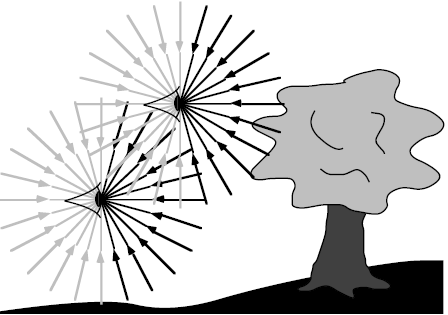
\includegraphics[width = 4cm]{images/plenoptic.png}
	\end{columns}
	
\end{frame}

\begin{frame}[fragile]
	\frametitle{The 4D Light Field}
	
	\begin{itemize}[<+- | alert@+>]
		\item Reduce dimensions of $P$
		\item $L(u, v, s, t)$
		\item Defined by two planes
	\end{itemize}
	\begin{center}
		\visible<3>{\documentclass{standalone}
\usepackage{tikz}

\begin{document}
	
	\begin{tikzpicture}[scale = 0.4]
	
		\filldraw[draw = black, fill = white] (0, 0) -- (5, -2) -- (5, 5) -- (0, 7) -- cycle;
		\filldraw[draw = black, fill = white] (9, 3) -- (14, 1) -- (14, 8) -- (9, 10) -- cycle;
		
		\draw[<-] (-3, 4) -- (1, 4);
		\draw (5, 4) -- (11, 4);
		\draw (14, 4) -- (17, 4);
		
		\node [left] at (-3, 4) {$L(u, v, s, t)$};
		
		
		\draw[fill] (1, 4) circle [radius = 0.1];
		\draw[fill] (11, 4) circle [radius = 0.1];
		
		\node[below right] at (1, 4) {$(u, v)$};
		\node[below right] at (11, 4) {$(s, t)$};
	
	\end{tikzpicture}
	
\end{document}}
	\end{center}
\end{frame}

\begin{frame}[fragile]
	\frametitle{Light Field Acquisition}
	
	\begin{itemize}[<+- | alert@+>]
		\item Camera array
		\item Camera gantry
		\item Plenoptic camera
	\end{itemize}
	
	\begin{center}
		\visible<1,2,3>{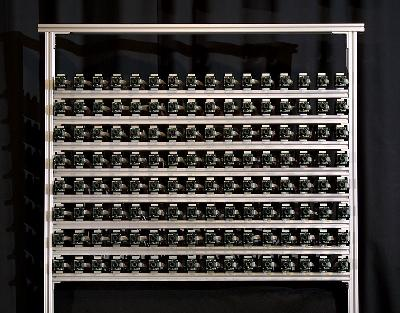
\includegraphics[height = 3.1cm]{images/stanford_camera_array_2.jpg}}
		\hspace{0.2cm}
		\visible<2, 3>{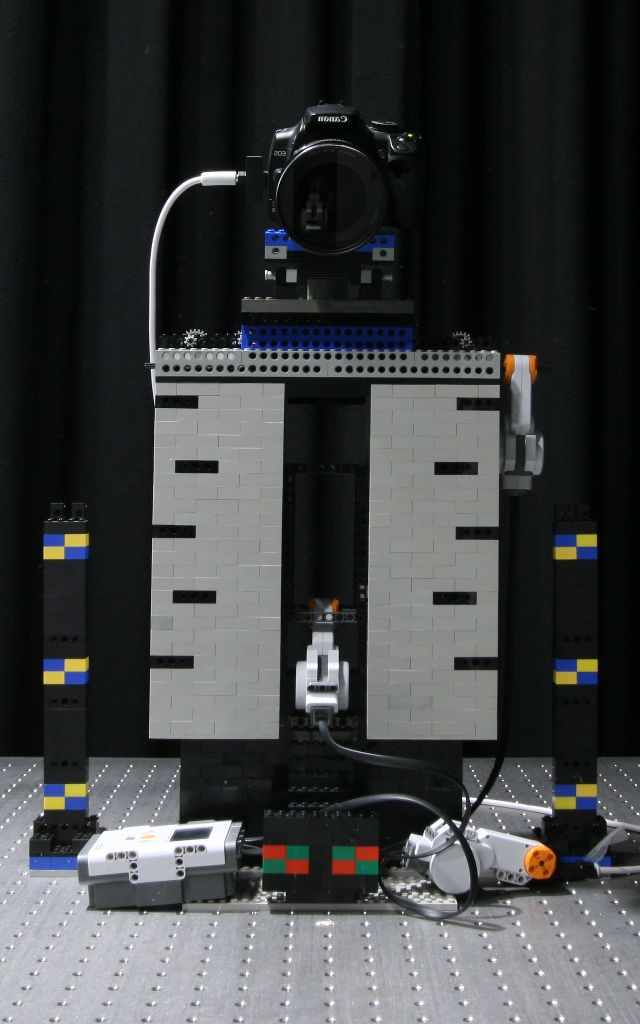
\includegraphics[height = 3.1cm]{images/lego_camera_gantry}}
		\hspace{0.2cm}
		\visible<3>{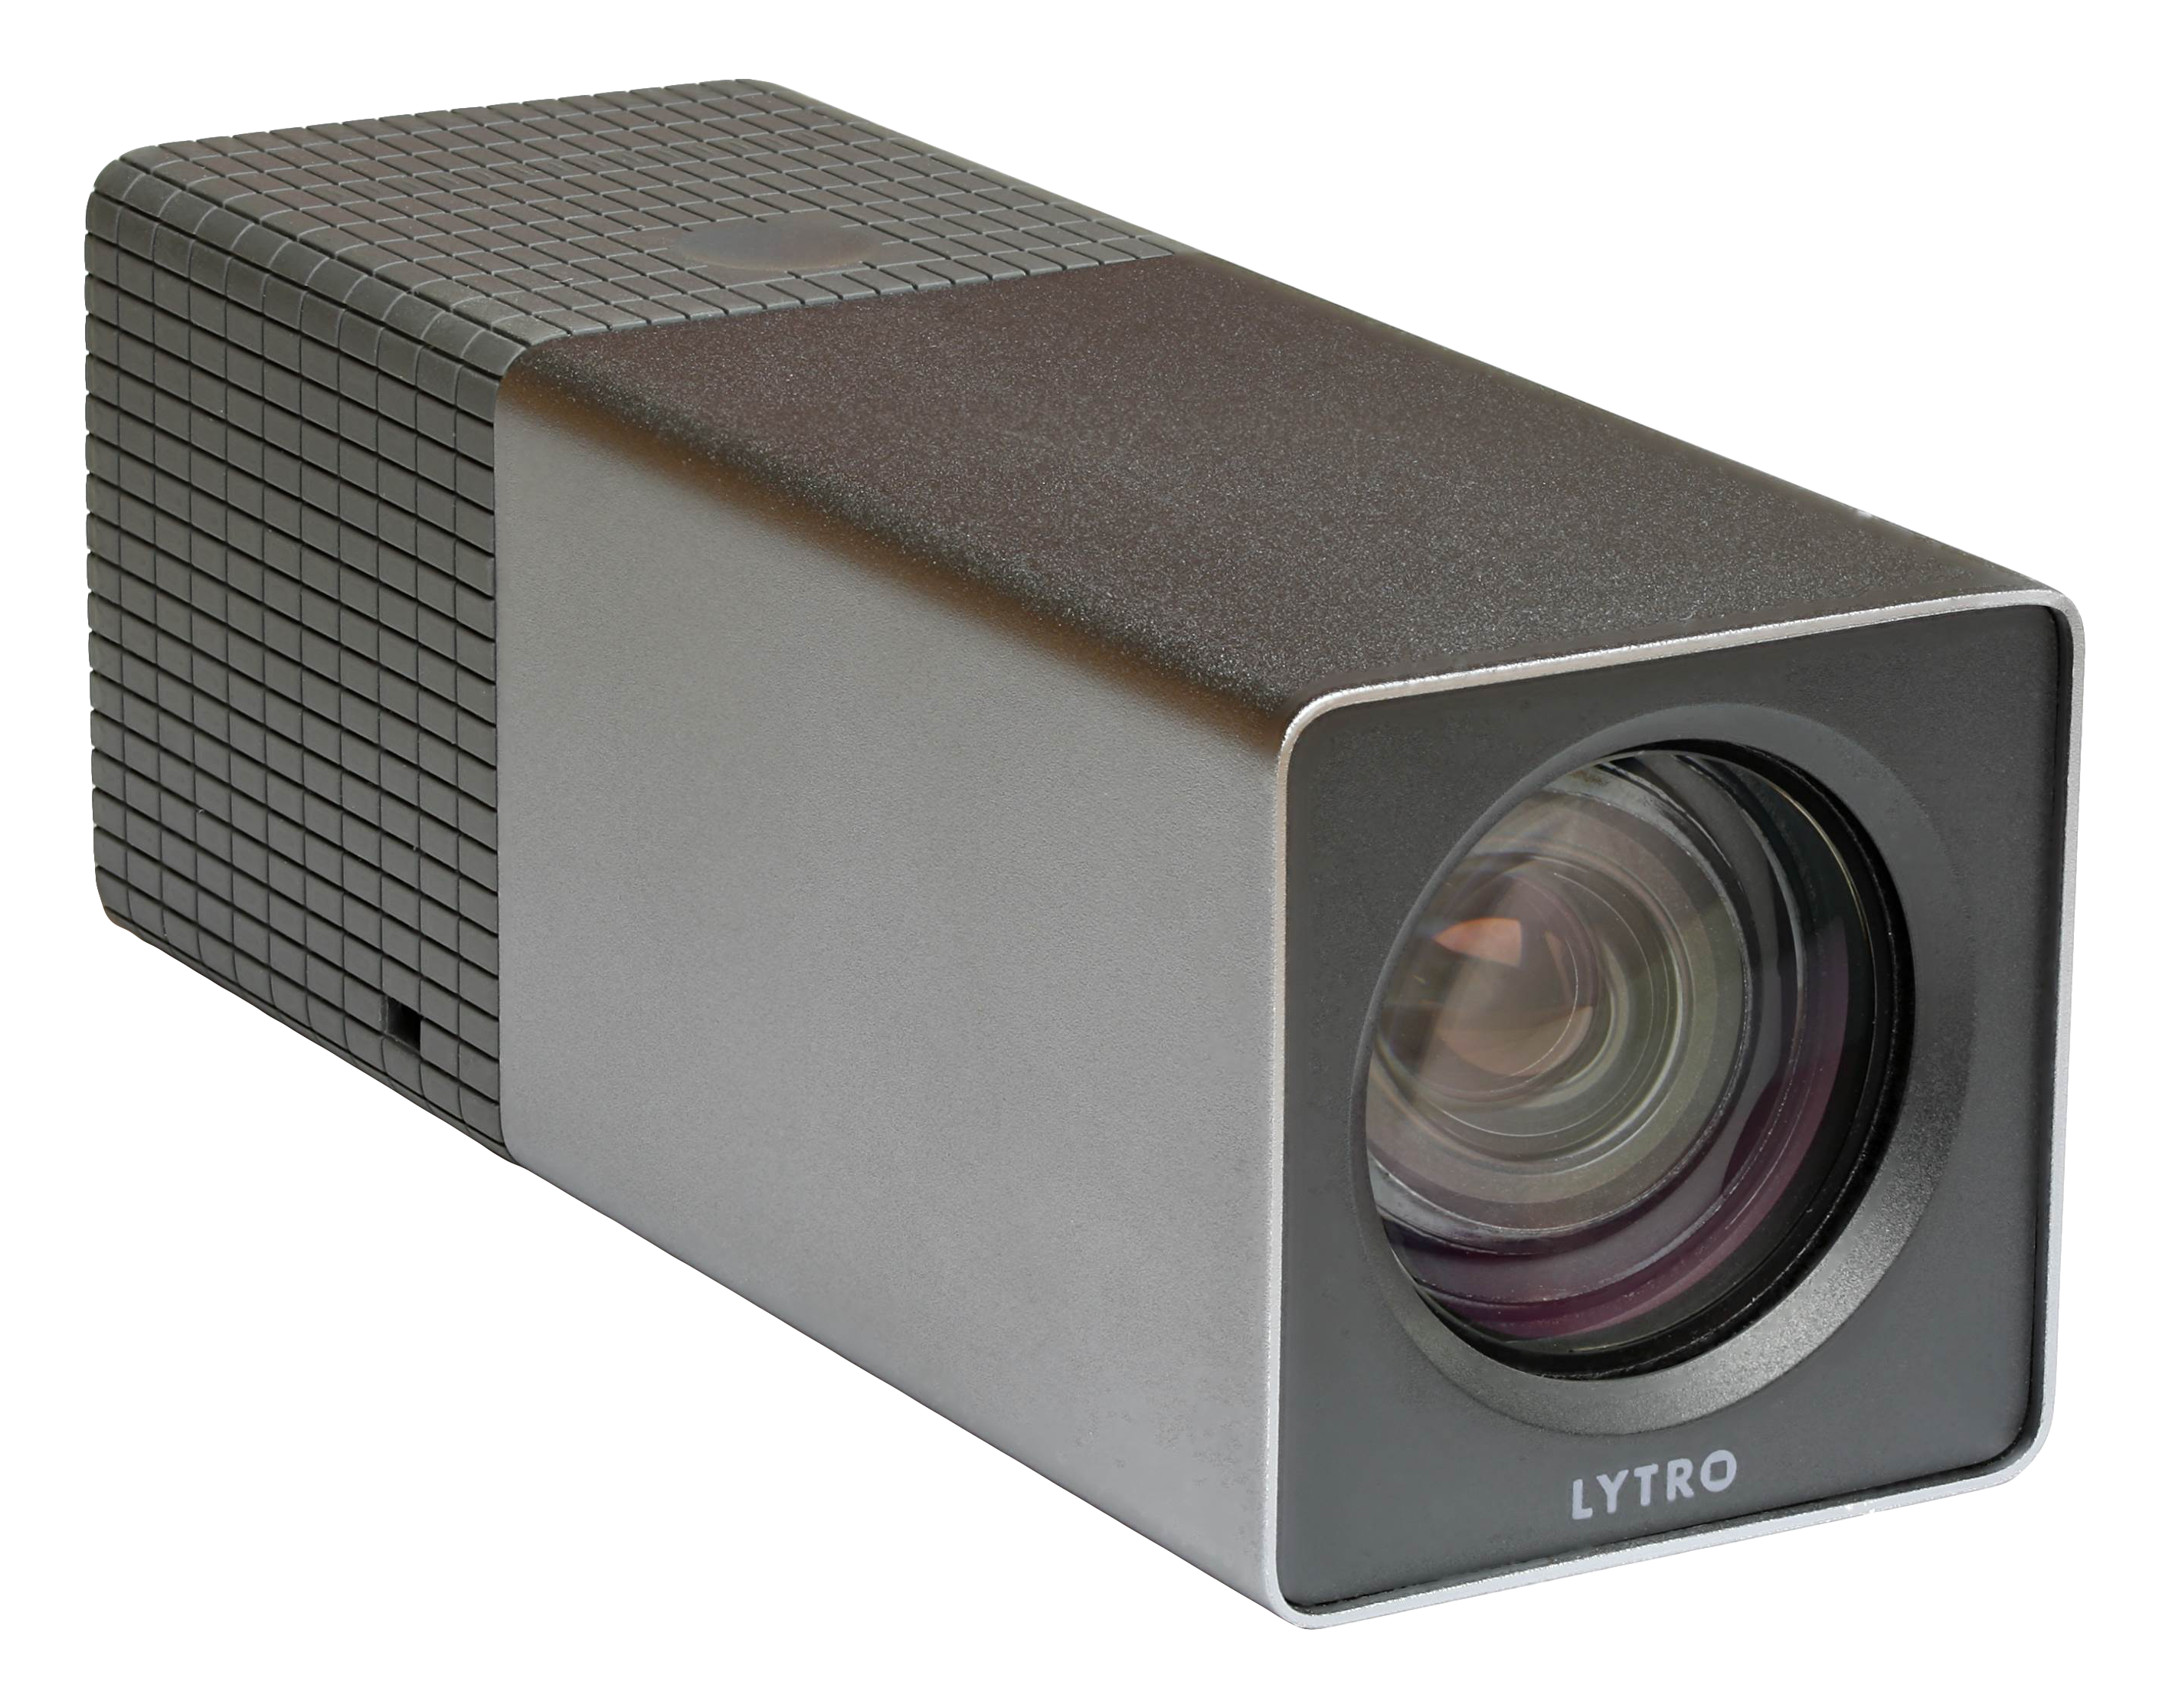
\includegraphics[height = 3.1cm]{images/Lytro_Light_Field_Camera-front_background_removed.png}}
	\end{center}
	
\end{frame}

\section{Problem Statement}
\begin{frame}[fragile]
	\frametitle{Optimization Problem}
	\begin{equation*} \label{eq:minimize_norm}
		\begin{aligned}
		& \underset{\alpha}{\text{argmin}} 	& & \left\lVert P \alpha + \bar{L} \right\rVert ^2 \\
		& \text{subject to} 				& & \alpha \geq 0.
		\end{aligned}
	\end{equation*}
\end{frame}
\section{Solution}
\section{Assessment}
\section{Conclusion}


\begin{frame}[fragile]
  \frametitle{mtheme}

  The \emph{mtheme} is a Beamer theme with minimal visual noise inspired by the
  \href{https://github.com/hsrmbeamertheme/hsrmbeamertheme}{\textsc{hsrm} Beamer
  Theme} by Benjamin Weiss.

  Enable the theme by loading

  \begin{minted}[fontsize=\small]{latex}
    \documentclass{beamer}
    \usetheme{m}
  \end{minted}

  Note, that you have to have Mozilla's \emph{Fira Sans} font and XeTeX
  installed to enjoy this wonderful typography.
\end{frame}

%\note[itemize]{
%	\item Note 1
%	\item Note 2
%}

\begin{frame}[fragile]
  \frametitle{Sections}
  Sections group slides of the same topic

  \begin{minted}[fontsize=\small]{latex}
    \section{Elements}
  \end{minted}

  for which the \emph{mtheme} provides a nice progress indicator \ldots
\end{frame}

\section*{Elements}

\begin{frame}[fragile]
  \frametitle{Typography}
      \begin{minted}[fontsize=\small]{latex}
The theme provides sensible defaults to \emph{emphasis}
text, \alert{accent} parts or show \textbf{bold} results.
      \end{minted}

  \begin{center}becomes\end{center}

  The theme provides sensible defaults to \emph{emphasis} text,
  \alert{accent} parts or show \textbf{bold} results.
\end{frame}
\begin{frame}{Lists}
  \begin{columns}[onlytextwidth]
    \column{0.5\textwidth}
      Items
      \begin{itemize}
        \item Milk \item Eggs \item Potatos
      \end{itemize}

    \column{0.5\textwidth}
      Enumerations
      \begin{enumerate}
        \item First, \item Second and \item Last.
      \end{enumerate}
  \end{columns}
\end{frame}
\begin{frame}{Descriptions}
  \begin{description}
    \item[PowerPoint] Meeh.
    \item[Beamer] Yeeeha.
  \end{description}
\end{frame}
\begin{frame}{Animation}
  \begin{itemize}[<+- | alert@+>]
    \item \alert<4>{This is\only<4>{ really} important}
    \item Now this
    \item And now this
  \end{itemize}
\end{frame}
\begin{frame}{Figures}
  \begin{figure}
    \newcounter{density}
    \setcounter{density}{20}
    \begin{tikzpicture}
      \def\couleur{mLightBrown}
      \path[coordinate] (0,0)  coordinate(A)
                  ++( 90:5cm) coordinate(B)
                  ++(0:5cm) coordinate(C)
                  ++(-90:5cm) coordinate(D);
      \draw[fill=\couleur!\thedensity] (A) -- (B) -- (C) --(D) -- cycle;
      \foreach \x in {1,...,40}{%
          \pgfmathsetcounter{density}{\thedensity+20}
          \setcounter{density}{\thedensity}
          \path[coordinate] coordinate(X) at (A){};
          \path[coordinate] (A) -- (B) coordinate[pos=.10](A)
                              -- (C) coordinate[pos=.10](B)
                              -- (D) coordinate[pos=.10](C)
                              -- (X) coordinate[pos=.10](D);
          \draw[fill=\couleur!\thedensity] (A)--(B)--(C)-- (D) -- cycle;
      }
    \end{tikzpicture}
    \caption{Rotated square from
    \href{http://www.texample.net/tikz/examples/rotated-polygons/}{texample.net}.}
  \end{figure}
\end{frame}
\begin{frame}{Tables}
  \begin{table}
    \caption{Largest cities in the world (source: Wikipedia)}
    \begin{tabular}{lr}
      \toprule
      City & Population\\
      \midrule
      Mexico City & 20,116,842\\
      Shanghai & 19,210,000\\
      Peking & 15,796,450\\
      Istanbul & 14,160,467\\
      \bottomrule
    \end{tabular}
  \end{table}
\end{frame}
\begin{frame}{Blocks}

  \begin{block}{This is a block title}
    This is soothing.
  \end{block}

\end{frame}
\begin{frame}{Math}
  \begin{equation*}
    e = \lim_{n\to \infty} \left(1 + \frac{1}{n}\right)^n
  \end{equation*}
\end{frame}
\begin{frame}{Quotes}
  \begin{quote}
    Veni, Vidi, Vici
  \end{quote}
\end{frame}

\plain{Dark background}{\vspace{-2em}\begin{center}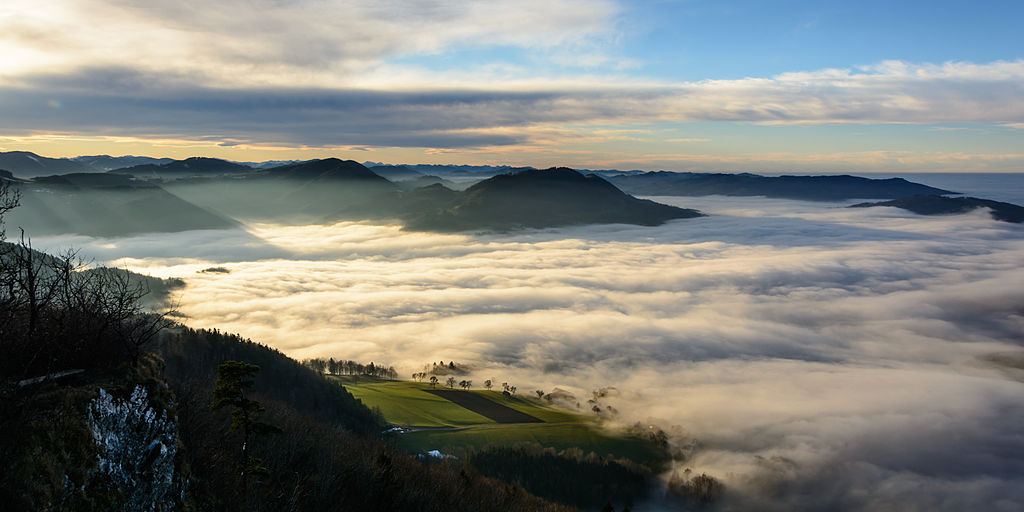
\includegraphics[width=\textwidth]{images/valley.jpg}\end{center}}

\section*{Conclusion}

\begin{frame}{Summary}

  Get the source of this theme and the demo presentation from

  \begin{center}\url{github.com/matze/mtheme}\end{center}

  The theme \emph{itself} is licensed under a
  \href{http://creativecommons.org/licenses/by-sa/4.0/}{Creative Commons
  Attribution-ShareAlike 4.0 International License}.

  \begin{center}\ccbysa\end{center}

\end{frame}

\plain{}{Questions?}

\end{document}
